\documentclass[12pt]{article}

\input{hw-preamble}

\begin{document}
\thispagestyle{empty}
\hw{2}{17 September 2023}

\problem Use minmax search to assign utility values for each internal node (i.e., non-leaf node) and indicate which path is the optimal solution for the MAX node at the root of the tree. Assume you explore the successors from left to right.

\solution
The optimal path is highlighted in Red.
\begin{figure}[!ht]
    \centering
    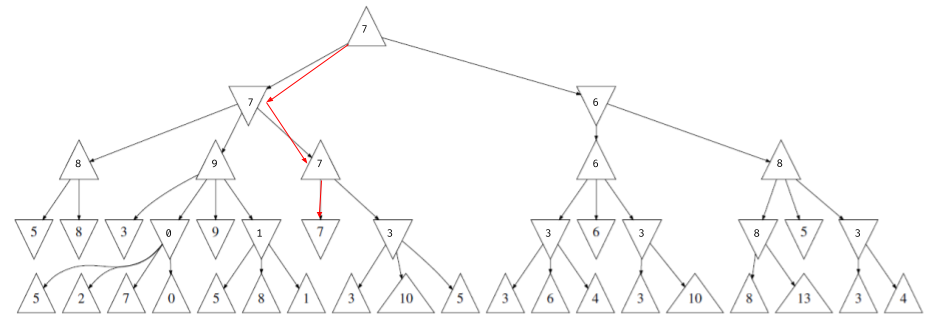
\includegraphics[width=\textwidth]{Images/Question 1.png}
    \caption{MinMax Search}
\end{figure}

\newpage
\problem Using the following figure 2, use $\alpha-\beta$ pruning to (1) assign utility values for each internal node (i.e., non-leaf node) and indicate which path is the optimal solution for the MAX node at the root of the tree. (2) For each node, indicate the final $\alpha$ and $\beta$ values. (3) For each cut that happens, draw a line to cross out that subtree.

\solution
The optimal path is highlighted in Red. Cuts are made with red lines.
\begin{figure}[!ht]
    \centering
    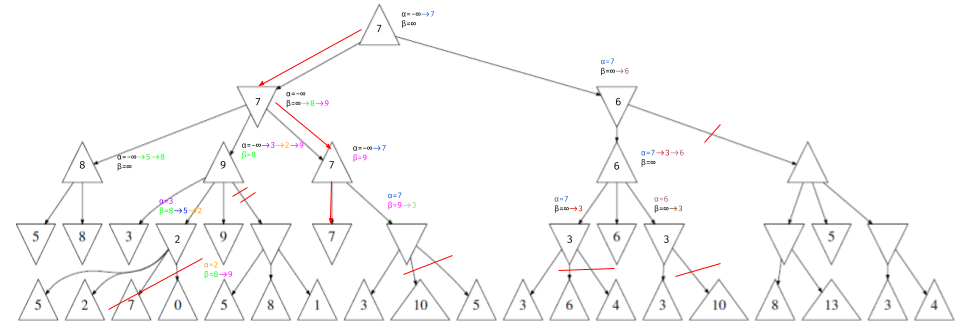
\includegraphics[width=\textwidth]{Images/Question 2.png}
    \caption{$\alpha-\beta$ pruning}
\end{figure}

\problem In Minmax search, we used a depth-first exploration through the use of recursion. We know that Minmax gives an optimal solution, however, we also know that depth-first search is suboptimal. Explain why Minmax gives an optimal solution even when it is using a depth-first exploration.

\solution
MinMax explores the entire game tree, considering all possible moves and counter-moves up to a certain depth or until the game ends.\\
This means that it does not miss any potential moves, ensuring a complete search of the state space.

\newpage
\problem Using a truth table, show that the resolution inference rule is valid. Note: valid means
``true under all interpretations".
\[\frac{P\lor Q,\lnot Q\lor R}{P\lor R}\]

\solution The Truth Table is as follows.

\begin{table}[!ht]
    \centering
    \begin{tabular}{|c|c|c||c|c|c|c||c|}
        \hline
        $P$ & $Q$ & $R$ & $(P\lor Q)$ & $(\lnot Q\lor R)$ & $(P\lor Q)\land(\lnot Q\lor R)$ & $(P\lor R)$ & $(P\lor Q)\land(\lnot Q\lor R)\rightarrow(P\lor R)$ \\ \hline
        T   & T   & T   & T           & T                 & T                               & T           & \textbf{T}                                          \\ \hline
        T   & T   & F   & T           & F                 & F                               & T           & \textbf{T}                                          \\ \hline
        T   & F   & T   & T           & T                 & T                               & T           & \textbf{T}                                          \\ \hline
        T   & F   & F   & T           & T                 & T                               & T           & \textbf{T}                                          \\ \hline
        F   & T   & T   & T           & T                 & T                               & T           & \textbf{T}                                          \\ \hline
        F   & T   & F   & T           & F                 & F                               & F           & \textbf{T}                                          \\ \hline
        F   & F   & T   & F           & T                 & F                               & T           & \textbf{T}                                          \\ \hline
        F   & F   & F   & F           & T                 & F                               & F           & \textbf{T}                                          \\ \hline
    \end{tabular}
    \caption{Truth Table}
\end{table}

\newpage
\problem In all of the problems in this section, show each step of the derivation and indicate which law (or other rules) you used: For example, \textit{distributive law, by definition, etc.}\\
\subproblem Convert $(Q\land\lnot P)\lor(Q\land R)\lor S$ into conjunctive normal form.

\solution Converting to CNF is as follows
\begin{flalign*}
    (Q\land \lnot P)\lor(Q\land R)\lor S & = (Q\land(\lnot P \lor R))\lor S      & \text{ Distributive Law} \\
                                         & = (Q\lor S)\land(\lnot P\lor R\lor S) & \text{ Distributive Law}
\end{flalign*}


\subproblem Convert $\lnot(\lnot P\lor Q)\lor R$ into conjunctive normal form.
\begin{flalign*}
    \lnot(\lnot P\lor Q)\lor R & = (\lnot\lnot P\land \lnot Q)\lor R & \text{ De Morgan Law}    \\
                               & = (P\land\lnot Q)\lor R             & \text{ Double Neggation} \\
                               & = (P\lor R)\land(\lnot Q\lor R)     & \text{ Distributive Law}
\end{flalign*}

\subproblem Convert $\lnot((\lnot P\rightarrow Q)\land(R\lor S))$ into the disjunctive normal form.
\begin{flalign*}
    \lnot((\lnot P\rightarrow Q)\land(R\lor S)) & = \lnot((\lnot\lnot P\lor Q)\land(R\lor S))      & \text{ Implication}     \\
                                                & = \lnot((P\lor Q)\land(R\lor S))                 & \text{ Double Negation} \\
                                                & = \lnot(P\lor Q)\lor\lnot(R\lor S)               & \text{ De Morgan's Law} \\
                                                & = (\lnot P\land\lnot Q)\lor(\lnot R\land\lnot S) & \text{ De Morgan's Law} \\
\end{flalign*}

\newpage
\problem Using resolution, show that $Q\lor W$ is a logical consequence of the following premises:
\begin{enumerate}
    \item $R\rightarrow W$
    \item $R\lor(\lnot P\land S)$
    \item $S\rightarrow(P\lor Q)$
    \item $S\lor R$
\end{enumerate}

\noindent
Transform the above problem into a set of clauses (premises and the conclusion), suitable for resolution-based theorem proving.

\solution The clauses are as follows:
\begin{enumerate}[C1.]
    \item $\lnot R\lor W$
    \item $R\lor\lnot P$
    \item $R\lor S$
    \item $\lnot S\lor(P\lor Q)$
    \item $S\lor R$
    \item $\lnot Q$
    \item $\lnot W$
\end{enumerate}

\problem Use resolution to derive False. Show every step. DO NOT USE any other inference rule.

\solution
C8. Resolve C4 and C6 on $Q$: $\neg S\lor P$ \\
C9. Resolve C5 and C8 on $S$: $R\lor P$
C10. Resolve C2 and C9 on $P$: $R$\\
C11. Resolve C1 and C10 on $R$: $W$\\
C12. Resolve C11 and C7 on $W$: $False$

\newpage
\problem Convert to prenex normal form
\begin{enumerate}
    \item $\lnot\forall x((\exists yQ(x,y))\rightarrow P(x))$
    \item $\forall x\lnot(\exists y Q(x,y)\land \lnot R(x))$
    \item $\lnot\exists x(\lnot(\forall yQ(x,y))\lor\lnot P(x))$
\end{enumerate}

\solution For expression 1.
\begin{flalign*}
    \lnot\forall x((\exists yQ(x,y))\rightarrow P(x)) & = \lnot\forall x(\lnot(\exists yQ(x,y))\lor P(x)) & \\
                                                      & = \lnot\forall x(\forall y\lnot Q(x,y)\lor P(x))  & \\
                                                      & = \exists x\lnot(\forall y\lnot Q(x,y)\lor P(x))  & \\
                                                      & = \exists x\exists y\lnot(\lnot Q(x,y)\lor P(x))  & \\
                                                      & = \exists x\exists yQ(x,y)\land \lnot P(x)        & \\
\end{flalign*}

\noindent
For expression 2.
\begin{flalign*}
    \forall x\lnot(\exists y Q(x,y)\land \lnot R(x)) & = \forall x\forall y \lnot(Q(x,y)\land \lnot R(x)) & \\
                                                     & = \forall x\forall y \lnot Q(x,y)\lor R(x)         &
\end{flalign*}

\noindent
For expression 3.
\begin{flalign*}
    \lnot\exists x(\lnot(\forall yQ(x,y))\lor\lnot P(x)) & = \lnot\exists x(\exists y \lnot Q(x,y)\lor\lnot P(x)) & \\
                                                         & = \forall x\lnot(\exists y \lnot Q(x,y)\lor\lnot P(x)) & \\
                                                         & = \forall x\forall y Q(x,y)\land P(x)
\end{flalign*}

\newpage
\problem Skolemize the expressions
\begin{enumerate}
    \item $\exists xP(x)$
    \item $\forall x\exists yP(x,y)$
    \item $\exists x\exists y\forall zP(x,y)\land Q(y,z)$
    \item $\forall x\exists y\exists zP(x,y,z)\land Q(y,z)$
    \item $\forall x\forall y\exists zP(x,y)\land Q(x,y,z)$
\end{enumerate}

\solution Skolemization  is as follows
\begin{enumerate}
    \item $P(\alpha )$
    \item $\forall xP(x,f(x))$
    \item $\forall zP(\alpha,\beta)\land Q(\beta,z)$
    \item $\forall xP(x,f(x),g(x))\land Q(f(x),g(x))$
    \item $\forall x\forall yP(x,y)\land Q(x,y,f(x,y))$
\end{enumerate}

\newpage
\problem Convert the following into a standard form (prenex, CNF, skolemization)
\[\forall x[\lnot(\exists z(P(z)\land Q(x,z)))\rightarrow\exists yR(x,y)]\]

\solution
Prenex
\begin{flalign*}
    \forall x[\lnot(\exists z(P(z)\land Q(x,z)))\rightarrow\exists yR(x,y)] & = \forall x[\exists z(P(z)\land Q(x,z))\lor \exists yR(x,y)]               & \\
                                                                            & = \forall x[(\exists zP(z) \land \exists zQ(x,z)) \lor \exists yR(x,y)]    & \\
                                                                            & = \forall x \exists z \exists u[(P(z) \land Q(x,u)) \lor \exists yR(x,y)]  & \\
                                                                            & = \forall x \exists z \exists u \exists y[(P(z) \land Q(x,u)) \lor R(x,y)]
\end{flalign*}

\noindent
CNF
\[\forall x \exists z \exists u \exists y[(P(z) \lor R(x,y)) \land (Q(x,u) \lor R(x,y))]\]

\noindent
Skolemization
\[\forall x [(P(f(x)) \lor R(x,g(x))) \land (Q(x,h(x)) \lor R(x,g(x)))]\]

\problem Apply the following substitutions to the expressions
\begin{enumerate}
    \item Apply $\{x/f(A)\}$ to $P(x,y)\lor Q(x)$.
    \item Apply $\{x/A,y/f(z)\}$ to $P(x,y)\lor Q(x)$.
    \item Apply $\{y/x\}$ to $P(x,y)\lor Q(x)$.
\end{enumerate}

\solution The substitutions are as follows:
\begin{enumerate}
    \item $P(f(A),y)\land Q(f(A))$
    \item $P(A,f(z))\land Q(A)$
    \item $P(x,x)\land Q(x)$
\end{enumerate}

\newpage
\problem For each of the following, (1) find the unifier, and (2) show the unified expression. For example, given $P(A)$ and $P(x)$, the unifier would be $\{x/A\}$, and the unified expression $P(A)$. If the pair of expressions is not unifiable, indicate so.
\begin{enumerate}
    \item $P(x,f(x),y)$ and $P(A,f(g(w)),z)$
    \item $P(x,A)$ and $P(y,y)$
    \item $P(x,f(g(x)),g(A),w)$ and $P(A,f(y),y,y)$
    \item $P(x,f(x))$ and $P(A,f(B))$
\end{enumerate}

\solution The unifier and unified expression are as follows:
\begin{enumerate}
    \item $P(x,f(x),y)$ and $P(A,f(g(w)),z)$
          \begin{enumerate}[(1)]
              \item $\{A/x\}$:\\
                    $P(x,f(x),y)$\\
                    $P(x,f(g(w)),z)$

              \item $\{x/g(w)\}$:\\
                    $P(x,f(g(w)),y)$\\
                    $P(x,f(g(w)),z)$

              \item $\{y/z\}$:\\
                    $P(x,f(g(w)),z)$\\
                    $P(x,f(g(w)),z)$
          \end{enumerate}

          \noindent
          Unifiers: $\{A/x,x/g(w),y/z\}$\\
          Unified Expression: $P(x,f(g(w)),z)$

          \newpage
    \item $P(x,A)$ and $P(y,y)$
          \begin{enumerate}[(1)]
              \item $\{A/x\}$:\\
                    $P(x,x)$\\
                    $P(y,y)$

              \item $\{x/y\}$:\\
                    $P(y,y)$\\
                    $P(y,y)$
          \end{enumerate}

          \noindent
          Unifiers: $\{A/x,x/y\}$\\
          Unified Expression: $P(y,y)$

    \item $P(x,f(g(x)),g(A),w)$ and $P(A,f(y),y,y)$
          \begin{enumerate}
              \item $\{A/x\}$:\\
                    $P(x,f(g(x)),g(x),w)$\\
                    $P(x,f(y),y,y)$

              \item $\{w/y\}$:\\
                    $P(x,f(g(x)),g(x),y)$\\
                    $P(x,f(y),y,y)$

              \item $\{y/g(x)\}$:\\
                    $P(x,f(g(x)),g(x),g(x))$\\
                    $P(x,f(g(x)),g(x),g(x))$
          \end{enumerate}

          \noindent
          Unifiers: $\{A/x,w/y,y/g(x)\}$\\
          Unified Expression: $P(x,f(g(x)),g(x),g(x))$

    \item $P(x,f(x))$ and $P(A,f(B))$
          \begin{enumerate}[(1)]
              \item $\{A/B\}$:\\
                    $P(x,f(x))$\\
                    $P(B,f(B))$

              \item $\{B/x\}$:\\
                    $P(x,f(x))$\\
                    $P(x,f(x))$
          \end{enumerate}

          \noindent
          Unifiers: $\{A/B,B/x\}$\\
          Unified Expression: $P(x,f(x))$
\end{enumerate}

\end{document}
